\documentclass{article}
\usepackage{preamble}
\begin{document}
\title{Exploration in \GROOVE}
\author{Arend Rensink}
\date{August 2024}
\maketitle

\section*{Terminology}

\begin{description}
\item[Absence] Equivalent to \emph{absent depth}.

\item[Absent depth] The \emph{absent depth} of a state is the minimal transient depth of that state and all its transitive successors. It follows that the \emph{absent depth} is smaller than or equal to the \emph{transient depth}. As long as a state is not \emph{complete}, its \emph{absent depth} may decrease as a consequence of further exploration.

\item[Absent] A state or transition is \emph{absent} if it should not be considered to be part of the state space. In particular, a state is \emph{absent} if it is \emph{complete} and has positive \emph{absent depth}; a transition is \emph{absent} if its target state is \emph{absent}. It follows that an \emph{absent} state is always \emph{transient}. Whether or not a state or transition is \emph{absent} is independent of whether or not it is \emph{inner}.

\item[Closed] A state is \emph{closed} if it is not \emph{open}. A \emph{closed} state may or may not be \emph{complete}.

\item[Complete] A state is \emph{complete} if it is \emph{closed} and all transitive successors up to (but not necessarily including) the first \emph{steady} state are also \emph{closed}. This means that the status of the state is fully known; in particular, it is possible, on the basis of its successors, to decide whether the state is \emph{absent}.

\item[Public] A state or transition is \emph{public} if it is both \emph{outer} and \emph{present} (or, in other words, if it is neither \emph{inner} nor \emph{absent}).

\item[Final] A state is \emph{final} if exploration is considered to terminate after reaching it. For instance, if two control blocks are concatenated, the second comes into play after the exploration of the first has reached a final state; also, if a state space is wrapped in an atomic block, the only \emph{steady} states, apart from the \emph{initial} state, are the \emph{final} ones. In other words, \emph{final} has the typical meaning in (regular) automata. A \emph{final} state is certainly \emph{closed} and \emph{steady}; it may or may not have successors.

\item[Initial] A state is \emph{initial} if it is the start state for the exploration. Its \emph{prime} is \emph{steady}.

\item[Incomplete] A state is \emph{incomplete} if it is not \emph{complete}.

\item[Inner] A state is \emph{inner} if it is inside the atomic block that makes up the body of a recipe, and a transition is \emph{inner} if it is a step in the execution of a recipe. Hence, an \emph{inner} state is certainly \emph{transient}, but the inverse does not hold. An \emph{inner} state that is not \emph{closed} may still evolve into an \emph{outer} one as a consequence of further exploration.

\item[Open] A state is \emph{open} if its direct outgoing transitions are not fully known. It follows that an open state can become \emph{closed} through further exploration of its outgoing transitions.

\item[Outer] A state or transition is \emph{outer} if it is not \emph{inner}.

\item[Present.] A state or transition is \emph{present} if it is not \emph{absent}. For a state, this means that it either has \emph{absent depth} zero (in which case it will certainly remain \emph{present} under further exploration} or it is \emph{incomplete} (in which case it may become \emph{absent} if, upon becoming \emph{complete}, it has positive \emph{absent depth}).

\item[Prime] The \emph{prime} of a state is the version of that state when it is just discovered, and no outgoing transitions have been explored. Hence, the \emph{prime} is \emph{open}, and may be \tmph{transient} even though (because of further exploration) the state itself has become \emph{steady} because its \emph{transient depth} has decreased to zero.

\item[Public] A state or transition is \emph{public} if it is both \emph{outer} and \emph{present}.

\item[Steady] A state is \emph{steady} if it is not \emph{transient}.

\item[Transience] Equivalent to \emph{transient depth}.

\item[Transient] A state is \emph{transient} if it is inside an atomic block, meaning that it has a positive \emph{transient depth}. A \emph{transient} state may or may not be \emph{inner}. A transient state that is \emph{open} may still evolve into a \emph{steady} state as a consequence of further exploration.

\item[Transient depth] The \emph{transient depth} of a state is the number of (nested) atomic blocks that it is inside of. A state is \emph{steady} if and only if its \emph{transient depth} is zero; otherwise it is \emph{transient}. As long as a state is not \emph{closed}, its \emph{transient depth} may decrease as a consequence of further exploration.
\end{description}

Figure~\ref{fig:venn} shows these different concepts in relation to each other.

\begin{figure}
\centering
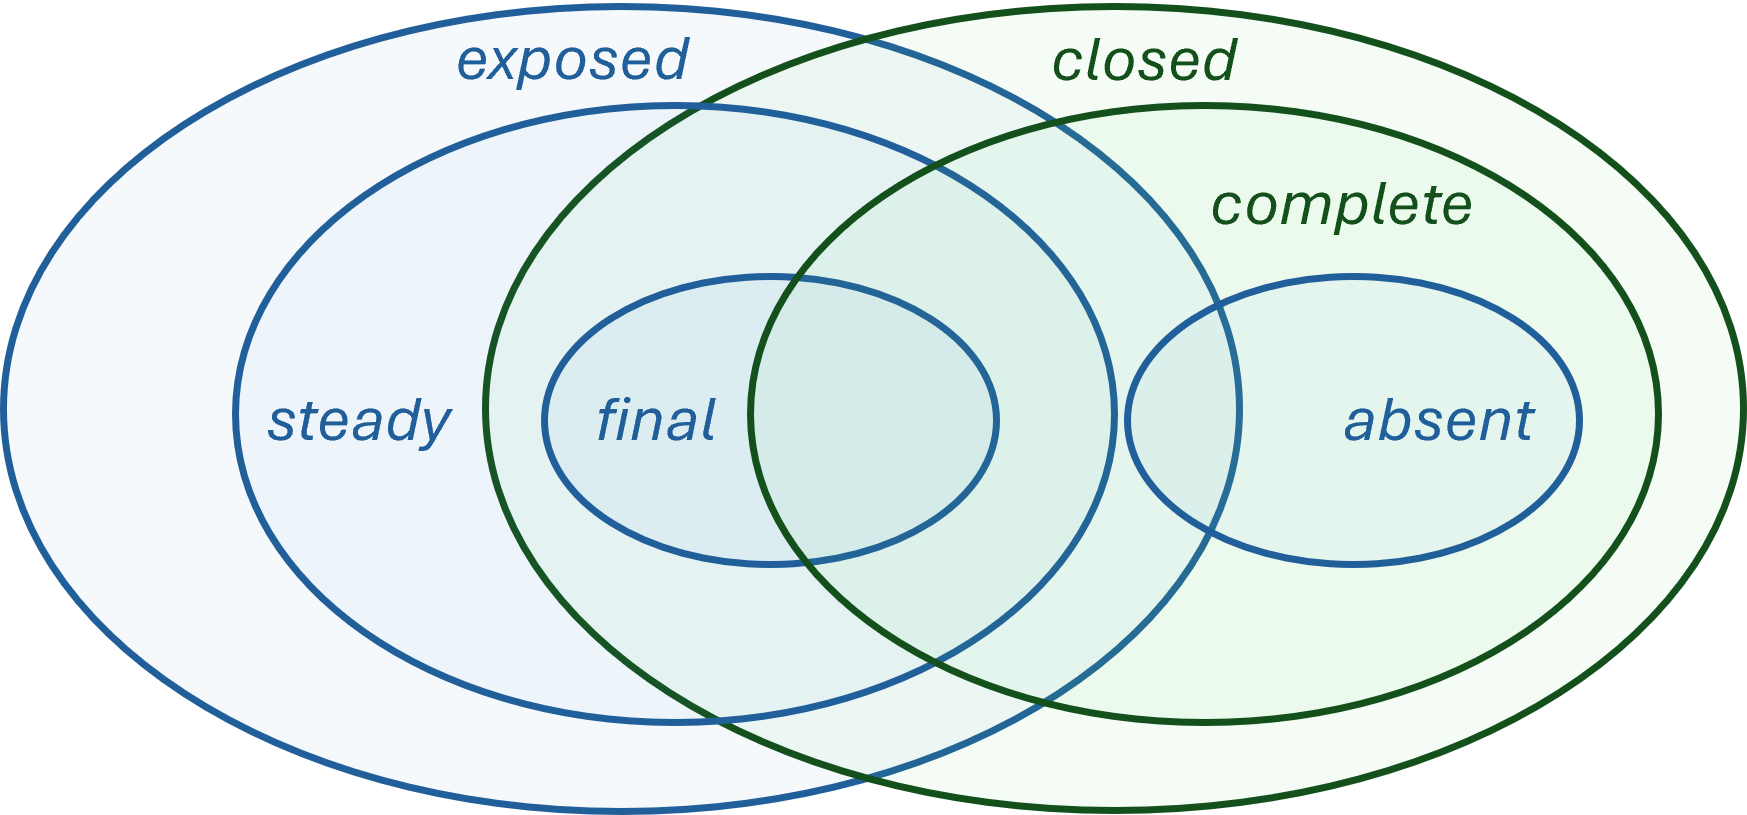
\includegraphics[scale=.5]{figs/venn}
\caption{Properties of states}
\label{fig:venn}
\end{figure}

\section*{Formalisation}

\medskip\noindent
We globally assume a set of labels $A$.

\medskip\noindent 
A state space is a tuple $\cS=\tupof{S,\iota,{\ra},{\up},\TDepth}$ with
\begin{itemize}
\item $S$ a set of states;
\item $\iota\in S$ the initial state;
\item ${\ra}\subseteq S\times A\times S$ a transition relation;
\item ${\up}\subseteq S$ a termination predicate;
\item ${\TDepth}:S\to \natN$ a \emph{transient depth} (or \emph{transience}) function.
\end{itemize}
%
State $s\in S$ is called \emph{final} if $p\up$, \emph{transient} (denoted $\Transient(s)$) if $\TDepth(s)>0$ and \emph{steady} (denoted $\Steady(s)$) if $\TDepth(s)=0$. There is a derived \emph{transaction relation}, which holds between all (pairs of) steady states for which there is a (non-empty) transition sequence that only passes through transient states.
%
\[ s\ttrans s' \enspace\iffdef\enspace
   s=s_0\trans{} s_1\trans{} \cdots \trans{} s_n=s' \:\wedge\:
   \setof{s_0,\ldots,s_n} \cap \Steady=\setof{s,s'}  \enspace.
\]
%
State spaces are generated from a \emph{pseudo-state spaces}.

\medskip\noindent
A pseudo-state space is a tuple $\cP=\tupof{P,\iota,{\mapsto},{\goesto},{\up},\TDepth}$ with
\begin{itemize}
\item $P$ a finite set of pseudo-states;
\item $\iota\in P$ the initial pseudo-state;
\item ${\step{}}\subseteq P\times A\times P$ a step relation;
\item ${\goesto}: P\times P$ an acyclic evolution relation;
\item ${\up} \subseteq P$ a termination predicate;
\item ${\TDepth}:P\to \natN$ a transient depth function.
\end{itemize}
%
Pseudo-state $p\in P$ is called \emph{prime} (denoted $\Prime(p)$) if $p\ncomesfrom$, \emph{closed} (denoted $\Closed(p)$) if $p\ngoesto$ and \emph{open} (denoted $\Open(p)$) if it is not closed.
%
A pseudo-state space is \emph{well-formed} if it satisfies the following additional properties:
\begin{itemize}
\item Stepping is deterministic; i.e., $\step{}$ is a partial function from $P$ to $A\times P$;
\item Evolution is deterministic; i.e., $\goesto$ is a partial function from $P$ to $P$;
\item Evolution is injective; i.e., $\comesfrom$ is a partial function from $P$ to $P$;
\item All steps go from open to prime pseudo-states; i.e., $p\step{}q$ implies $\Open(p)$ and $\Prime(q)$;
\item All final pseudo-states are steady and closed; i.e., $p\up$ implies $\Steady(p)$ and $\Closed(p)$;
\item Stepping cannot decrease transience; i.e., $p\step{}q$ implies $\TDepth(q)\geq \TDepth(p)$;
\item Evolution cannot increase transience; i.e., $p\goesto q$ implies $\TDepth(q)\leq \TDepth(p)$.
\end{itemize}
%
From now on, we only deal with well-formed pseudo-states spaces. The \emph{prime of} and \emph{closure of} a pseudo-state $p$ are defined as
%
\begin{align*}
	\prm p & = q \quad \text{where $\Prime (q)$ and $q\goesto^* p$} \\
	\cls p & = q \quad \text{where $p\goesto^* q$ and $\Closed(q)$} \enspace.
\end{align*}
%
Note that these are well-defined because $P$ is finite and $\goesto$ is acyclic, deterministic and injective (implying that it is a union of finite chains of pseudo-states). A pseudo-state space effectively represents a state space in which the states are $\goesto$-related sets of pseudo-states --- which, as remarked above, are actually chains. Rather than formalising the relation in this way, however, we let a state be represented by the initial element of such a chain, i.e., by the (unique) prime pseudo-state.

\medskip\noindent
Given a pseudo-state space $\cP$ as above, a \emph{configuration} is set $C\subseteq P$ of pseudo-states with $\iota\in C$ that is $\goesto$-left-closed (implying, among other things, that $\prm p\in C$ for all $p\in C$) and, moreover, $p\in C$ with $p\comesfrom\:\step q$ implies $q\in C$. (It follows that $P$ is itself a configuration of $\cP$.) Every configuration $C$ generates a state space $\cS_C= \tupof{S_C,\iota_C,\trans{}_C, \up_C, \TDepth_C}$ as follows:
%
\begin{align*}
S_C & = \gensetof{\prm p}{p\in C} \\
\iota_C & = \iota \\
{\trans{}_C} & = \gensetof{(\prm p,a,q)}{p,q\in C, p\step a q} \\
\up_C & = \gensetof{\prm p}{p\in C, p\up} \\
\TDepth_C & : p \mapsto \min \gensetof{\TDepth(q)}{q\in C,p=\prm q} \enspace \text{for all $p\in S_C$} \enspace.
\end{align*}
%
The notion of closure and stability are also extended to configurations (so as to coincide with their counterparts for $S_C$):
\begin{align*}
\Closed_C & = \gensetof{\prm p}{p\in C, p\ngoesto} \\
\Steady_C & = \gensetof{\prm p}{p\in C, \TDepth(p)=0} \enspace.
\end{align*}
%
We define some further auxiliary notions.
%
\begin{itemize}
\item $\Complete_C(s)$ for $s\in S_C$ expresses that $s$ as well as all its discovered $\trans{}_C$-successors are closed, up to and including the first steady state. It is defined as the smallest set such that
%
\[ \Complete_C = \Closed_C\cap \bigl(\Steady_C \cup \gensetof{p\in S_C}{\forall p\trans{}_C q.\, q\in \Complete_C\cup \Steady_C}\bigr) \enspace.
\]

\item $\ETDepth_C(s)$ for $s\in S_C$ is the \emph{eventual transient depth} in $C$, meaning the minimum transient depth of $s$ and all its $\trans{}_C$-successors. It is defined by
%
\[ \ETDepth_C: p\mapsto \min\gensetof{\TDepth(q)}{p\trans{}_C^* q} \text{ for all $p\in S_C$} \enspace. \]

\item $\ESteady_C(s)$ for $s\in S_C$ expresses that $s$ is \emph{eventually steady} in $C$, meaning that it or one of its discovered $\trans{}_C$-successors is steady (i.e., has transient depth 0). It is defined by
%
\[ \ESteady_C=\gensetof{p\in S_C}{\ETDepth_C(p)=0} \enspace. \]

\item $\Absent_C(s)$ for $s\in S_C$ expresses that $s$ is \emph{absent} in $C$, which is the case if it is complete (all reachable steady states have been discovered) but not eventually steady (no reachable steady state has been discovered). It is defined by
\[ \Absent_C=\Complete_C\setminus \ESteady_C \enspace. \]
\end{itemize}
%
We want to construct $S_P$ incrementally by approaching $P$ through a sequence of configurations, starting with $\setof{\iota}$ and adding, at each iteration, an evolution $p\goesto p'$ with $p\in C$ and $p'\notin C$. The latter is defined by 
\[ C\oplus(p\goesto p') = C\cup \setof{p'} \cup \gensetof{q}{p\step a q} \enspace. \]
Incremental construction means that, if $D=C\oplus(p\goesto p')$, all components of $S_D$ can be constructed from $S_C$ and $\cP$. Indeed, we have
%
\begin{align*}
\trans{}_D & = {\trans{}_C} \cup\gensetof{(\prm p,a,q)}{p\step a q} \\
\up_D & = \up_C \cup \gensetof{p'}{p'\up} \\
\TDepth_D & : s\mapsto
  \begin{cases}
  \TDepth(p') & \text{if $s=\prm p$} \\
  \TDepth(q) & \text{if $s=q\notin S_C$} \\
  \TDepth_C(s) & \text{otherwise}
  \end{cases} \\
\Closed_D & = \Closed_C \cup\gensetof{\prm p}{p'\ngoesto} \\
\Steady_D & = \Steady_C \cup \gensetof{\prm p}{\TDepth(p')=0} \enspace.
\end{align*}
%
For $\ttrans_C$, however, the case is less easy. For the purpose of this construction, we introduce several auxiliary data structures.

\begin{itemize}
\item A transition $t\trans{a}_C t$ is \emph{partial} if it starts in a $\cP$-transient state:
%
\[ \Partial_C = \gensetof{(s,a,t)\in {\trans{}_C}}{\Transient(s)} \]

\item 
%
\[ \RS_C : s \mapsto \gensetof{(t,a,t')\in \Partial_C}{\Transient(t), s\trans{}_C^* t\trans a_C t'} \]

\item For a given state $s$, the \emph{reachable transient open states} are the $C$-open states reachable through a (possibly empty) sequence of $\trans{}_C$-transitions between $\cP$-transient states.
%
\[ \RTO_C : s \mapsto \gensetof{t\in S_C\setminus \Closed_C}{s\trans{}_C^* t} \]

\end{itemize}
\end{document}
